\chapter{Introduction}

Current datasets are often generated through extensive experiments utilizing full-scale systems such as MilliAmpere. While these experiments are essential for specific research purposes, the cost-benefit ratio may not be proportional when the primary goal is to collect sensor data.

Identifying the lack of a low-threshold approach to data collection, I initiated the development of a human-operable \sr during my preproject. The objective was to create a lightweight \sr that addressed common challenges like synchronization and pose estimation, enabling a more accessible approach to high-quality data acquisition.

Most of the hardware and electronics work was completed durin my \preproject, but a lot of work remained on the software side.

\begin{figure}[H]
    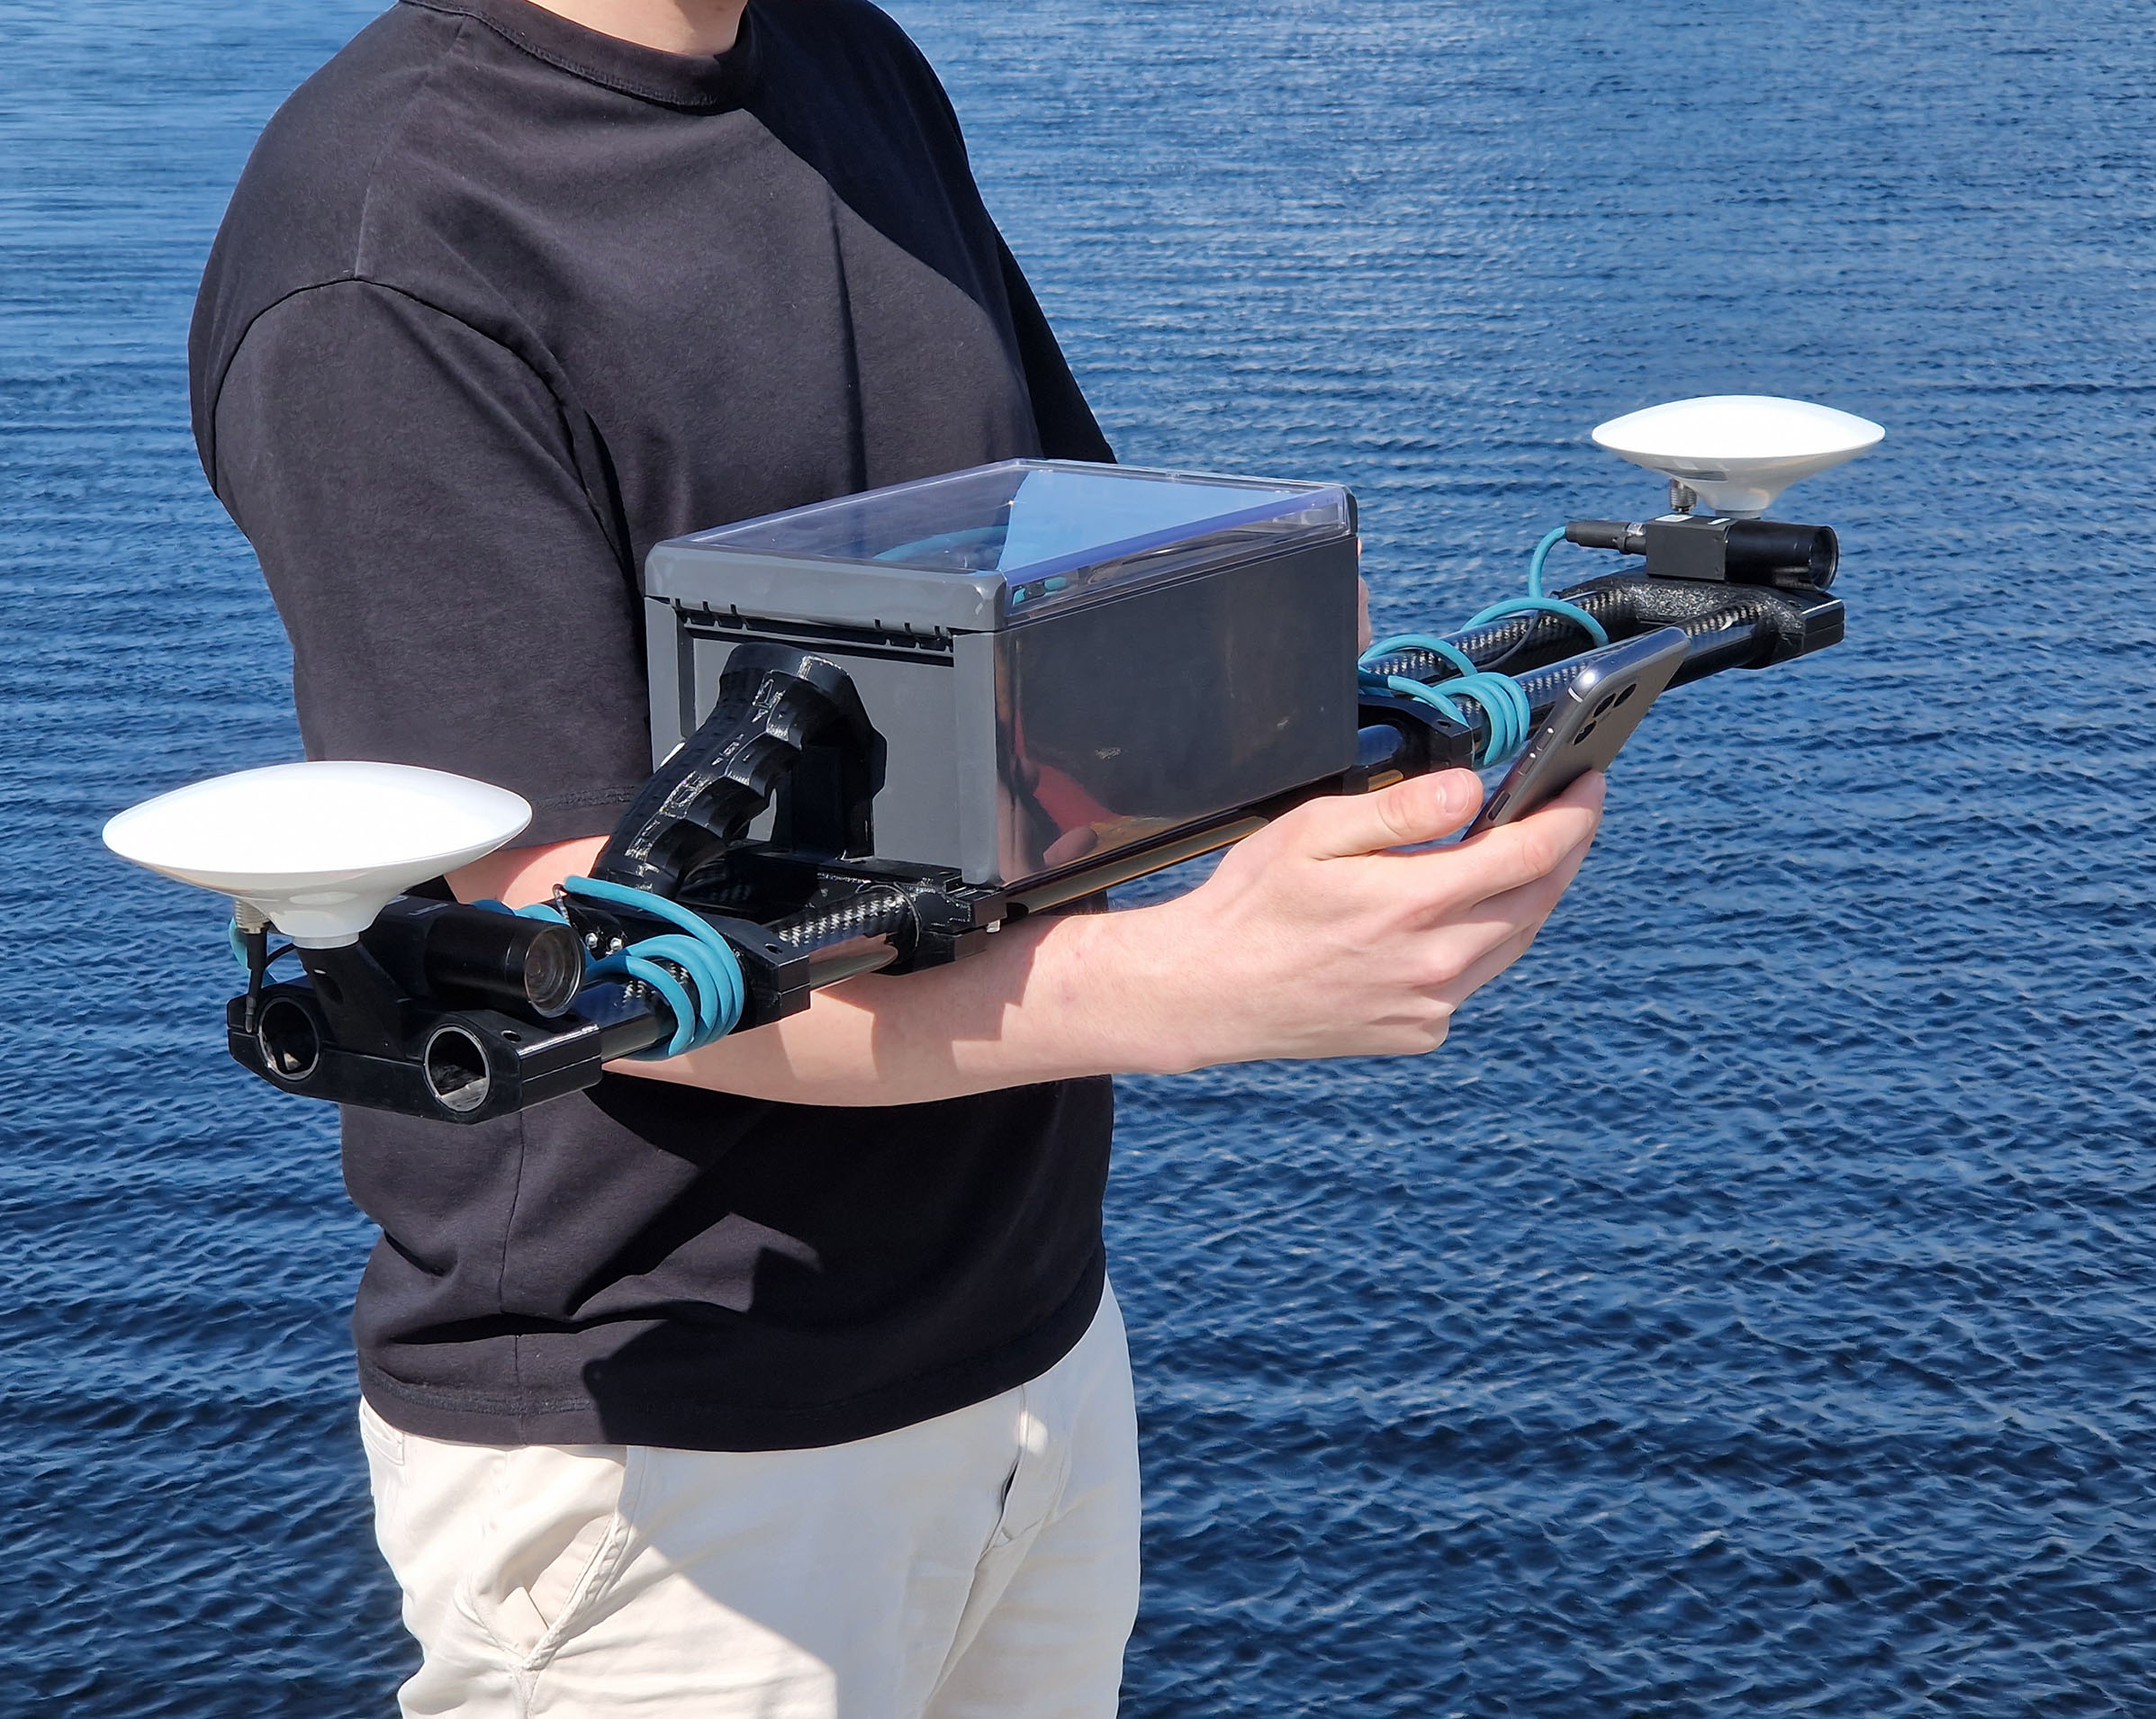
\includegraphics[width=\textwidth]{figures/frontpage.jpg}
    \caption{The Sensor Rig}
\end{figure}




program, where I will focus on investigating the potential enhancements in detection capabilities for Autonomous Surface Vessels (ASVs) through the integration of data from various sensors, such as lidars and specialized cameras.
This research will heavily involve machine learning techniques, necessitating a significant amount of training data.
Since I will be exploring new sensor combinations, existing datasets alone cannot fulfill the requirements.
Hence, there is a need for a framework that enables the collection of new data, with a preference for a low threshold approach.
Therefore, the development of this sensor rig becomes imperative.

Explain how this project is a bit all over the place but show how it ties together with a full page figure.


\section{Motivation}
A significant amout of work was put into enabling on-the-fly compression of the videostreams from the \sr.
That is the ability to compress the video data as it is being recorded, and storing the compressed data on disk.

The cameras on the \sr produce roughly $2Gb/s$ of data.
Aditionally, the \gls{imu} and \gls{gnss} produce data, but amount is neglible compared with the cameras.
At this rate it infeasable to record long datasets as almost a terrabyte of data is produced every hour.
\begin{align}
    \frac{1TB}{2Gb/s}  = \frac{8Tb}{2Gb/s} = 4000s \approx 1h + 7min
\end{align}

It is reasonable to say that a much easer option is to buy \gls{ssd} with a capacity up to 8TB \cite{CorsairMP600PRO}, enabling roughly 9 hours of recording.
One reason this
\cite{microntechnologyMicron2300SSD2020}


\subsection{Limited write speed}
One issue when storing the raw data at first was that the \jx was not able to write to the disk fast to the installed \gls{ssd}.
The write speed was tested using:
\begin{minted}[linenos=false]{bash}
    sudo dd if=/dev/zero of=./testfile bs=8k count=100k conv=fdatasync
\end{minted}
which repeatedly reported write speeds just below $2Gb/s$ (250MB).
This is weird, as the \gls{ssd} has a write speed of $2.7GB/s$, but other people have faced similar issues on the \jx \cite{microntechnologyMicron2300SSD2020} \cite{dtyuImbalancedPerformanceRead2018}.
This is probably fixable, but provides further motivation to enable on the fly compression

\subsection{Streaming to external devices}
Having a

\subsection{Integration with other systems}
The main intended purpose of the \sr is to be carried around by a human operator and



\section{Challenges}
The main challenge in this project has been to design a system that can effectively manage the large amount of raw data produced by the two cameras.
Each camera features a 5.0MP sensor configured to capture 10-bit raw images 16 times every second \cite{lucidvisionlabsTriton0MPPolarization}.
To put this into perspective, a single frame contains more data than what is needed to store the entire collection of William Shakespeare's works in plain text \cite{projectgutenbergCompleteWorksWilliam1994}.

If the output from these cameras were stored directly to disk, almost a Terabyte of data would be generated every hour, making it infeasible to collect long term data sets.
\section{Contributions}



\section{Outline}
Completing the \sr project has involved extensive work on various topics, ranging from hardware design and full stack web development to kernel compilation and low-level optimizations in CUDA.
Although some of the topics are closely related, others are only connected  by contributing towards the final product.

With this in mind it has been difficult to decide on a structure for this report and what to include.
In the end I decided to collect the software development theory in the first chapter, and dedicate a chapter to each of the major topics I have worked on with a focus on the practical aspects of the work, to serve as a referece for future work.

As some chapters might be less relevant depending on the reader's background, I have tried to make each chapter as self-contained as possible.
The following is a brief overview of the content of each chapter:

\paragraph{Chapter \ref{chap:programming_theory}: Real time programming on Jetson Xavier}
This chapter provides an overview of the theoretical background relevant to real-time performance on the Jetson Xavier platform and the development of real-time software in general. It explores topics such as real-time programming theory, performance considerations for heterogeneous systems, and introduces the CUDA programming model.

\paragraph{Chapter \ref{chap:cameras}: Polarization Cameras}
This chapter presents the special type of polarization cameras used, explain how they work and why they are particularly well suited for detection in marine environments.
Furthermore, it covers how to interact with the \cams through thair \gls{api} and how the network adapters have been configured to acheive reliable $2Gb/s$ throughput from the \cams.

\paragraph{Chapter \ref{chap:debayer}: Efficient processing of raw image bitstream in CUDA}
To make it possible to compress the video streams, the raw data has to be transformed into a format that can be processed by the \gls{h265} encoder.
This chapter explains how this is acheived in real time using CUDA.

\paragraph{Chapter \ref{chap:gstreamer}: Video Compression using GStreamer}
\gls{gstreamer} is a powerful framework for processing video streams.
This chapter explains how it is used to compress the video streams in real time using hardware accelration on the \jx.
It also covers how \gls{pygo} is used to interact with the \gls{gstreamer} pipeline from Python.

\paragraph{Chapter \ref{chap:pipeline}: Pipeline Assembly in Python}
The three previous chapters are tied together in this chapter, which explains how the various components are assembled into a working pipeline.

\paragraph{Chapter \ref{chap:gui}: Web Interface to Control, Monitor and Stream Video}
A web application was developed to enabling real time control and monitoring of the \sr and its video streams.
This allows anyone with a smartphone to operate the \sr without any prior training or technical knowledge.
In a ddition a \gls{pubsub} server was implemented for communication between the web application and the pipeline.

\paragraph{Chapter \ref{chap:flashing_xavier}: Compiling Jetson Linux with PPS}
This chapter presents a systematic approach to compile, flash and debug the \gls{os} on the \jx.
Updating the \gls{os} was necessary to get the \gls{gstreamer} pipeline working.
As a \gls{pps} suuport is requiered  to synchronize the clock on the \jx to \gls{utc}, it was necessary to configure the underlying Linux kernel to support this, which was more complicated than expected.

\paragraph{Chapter \ref{chap:hardware}: Improving the Hardware}
After the \preproject most of the hardware was already in place, but some parts were missing.
I applied for, and got, funding to purchase a new 3D printer to enable an iterateive design process.
With this in place custom ergonomic carry handles, new combined camera and antenna mounts and other minor parts were designed and 3D-printed.

\paragraph{Chapter \ref{chap:results}: Results}
With everything in place, the \sr was tested in the field.
Several smaller datasets are collected and visualization tools has been developed to facilitate analysis of the data.

\paragraph{Chapter \ref{chap:future_work}: Ongoing developments and future work}
Some design flaws from the \preproject remain to be fixed and a few possible performance improvements have been identified.
With the goal of creating a fully autonomous sensor rig acheived, the next step is to create state of the art stereo polarization datasets and advance the field of situational awareness for autonomous surface vessels.